% Options for packages loaded elsewhere
\PassOptionsToPackage{unicode}{hyperref}
\PassOptionsToPackage{hyphens}{url}
\PassOptionsToPackage{dvipsnames,svgnames,x11names}{xcolor}
%
\documentclass[
]{estat/estat}

\usepackage{amsmath,amssymb}
\usepackage{iftex}
\ifPDFTeX
  \usepackage[T1]{fontenc}
  \usepackage[utf8]{inputenc}
  \usepackage{textcomp} % provide euro and other symbols
\else % if luatex or xetex
  \usepackage{unicode-math}
  \defaultfontfeatures{Scale=MatchLowercase}
  \defaultfontfeatures[\rmfamily]{Ligatures=TeX,Scale=1}
\fi
\usepackage{lmodern}
\ifPDFTeX\else  
    % xetex/luatex font selection
    \setmainfont[]{Arial}
\fi
% Use upquote if available, for straight quotes in verbatim environments
\IfFileExists{upquote.sty}{\usepackage{upquote}}{}
\IfFileExists{microtype.sty}{% use microtype if available
  \usepackage[]{microtype}
  \UseMicrotypeSet[protrusion]{basicmath} % disable protrusion for tt fonts
}{}
\makeatletter
\@ifundefined{KOMAClassName}{% if non-KOMA class
  \IfFileExists{parskip.sty}{%
    \usepackage{parskip}
  }{% else
    \setlength{\parindent}{0pt}
    \setlength{\parskip}{6pt plus 2pt minus 1pt}}
}{% if KOMA class
  \KOMAoptions{parskip=half}}
\makeatother
\usepackage{xcolor}
\usepackage[left=3cm,right=2cm,top=3cm,bottom=2cm]{geometry}
\setlength{\emergencystretch}{3em} % prevent overfull lines
\setcounter{secnumdepth}{5}
% Make \paragraph and \subparagraph free-standing
\makeatletter
\ifx\paragraph\undefined\else
  \let\oldparagraph\paragraph
  \renewcommand{\paragraph}{
    \@ifstar
      \xxxParagraphStar
      \xxxParagraphNoStar
  }
  \newcommand{\xxxParagraphStar}[1]{\oldparagraph*{#1}\mbox{}}
  \newcommand{\xxxParagraphNoStar}[1]{\oldparagraph{#1}\mbox{}}
\fi
\ifx\subparagraph\undefined\else
  \let\oldsubparagraph\subparagraph
  \renewcommand{\subparagraph}{
    \@ifstar
      \xxxSubParagraphStar
      \xxxSubParagraphNoStar
  }
  \newcommand{\xxxSubParagraphStar}[1]{\oldsubparagraph*{#1}\mbox{}}
  \newcommand{\xxxSubParagraphNoStar}[1]{\oldsubparagraph{#1}\mbox{}}
\fi
\makeatother


\providecommand{\tightlist}{%
  \setlength{\itemsep}{0pt}\setlength{\parskip}{0pt}}\usepackage{longtable,booktabs,array}
\usepackage{calc} % for calculating minipage widths
% Correct order of tables after \paragraph or \subparagraph
\usepackage{etoolbox}
\makeatletter
\patchcmd\longtable{\par}{\if@noskipsec\mbox{}\fi\par}{}{}
\makeatother
% Allow footnotes in longtable head/foot
\IfFileExists{footnotehyper.sty}{\usepackage{footnotehyper}}{\usepackage{footnote}}
\makesavenoteenv{longtable}
\usepackage{graphicx}
\makeatletter
\def\maxwidth{\ifdim\Gin@nat@width>\linewidth\linewidth\else\Gin@nat@width\fi}
\def\maxheight{\ifdim\Gin@nat@height>\textheight\textheight\else\Gin@nat@height\fi}
\makeatother
% Scale images if necessary, so that they will not overflow the page
% margins by default, and it is still possible to overwrite the defaults
% using explicit options in \includegraphics[width, height, ...]{}
\setkeys{Gin}{width=\maxwidth,height=\maxheight,keepaspectratio}
% Set default figure placement to htbp
\makeatletter
\def\fps@figure{htbp}
\makeatother

\authors{%
    Bruno Boaventura Xavier\\

    
}

% escreva o nome do cliente aqui
% se for mais de um separe por \\
\client{%
    House of Excellence
}
% Baixando pacotes
\RequirePackage{fancyhdr}
\RequirePackage{graphicx}

\setlength\headheight{28pt}  

\setlength{\parindent}{15pt} % Adiciona indentação nos parágrafos
\setlength{\parskip}{0pt} % Adiciona 0 espaço entro os parágrafos

\newcommand{\estat}{\textbf{ESTAT}\xspace}
\newcommand{\direx}{\textbf{DIREX}\xspace}
\makeatletter
\@ifpackageloaded{caption}{}{\usepackage{caption}}
\AtBeginDocument{%
\ifdefined\contentsname
  \renewcommand*\contentsname{Índice}
\else
  \newcommand\contentsname{Índice}
\fi
\ifdefined\listfigurename
  \renewcommand*\listfigurename{Lista de Figuras}
\else
  \newcommand\listfigurename{Lista de Figuras}
\fi
\ifdefined\listtablename
  \renewcommand*\listtablename{Lista de Tabelas}
\else
  \newcommand\listtablename{Lista de Tabelas}
\fi
\ifdefined\figurename
  \renewcommand*\figurename{Figura}
\else
  \newcommand\figurename{Figura}
\fi
\ifdefined\tablename
  \renewcommand*\tablename{Tabela}
\else
  \newcommand\tablename{Tabela}
\fi
}
\@ifpackageloaded{float}{}{\usepackage{float}}
\floatstyle{ruled}
\@ifundefined{c@chapter}{\newfloat{codelisting}{h}{lop}}{\newfloat{codelisting}{h}{lop}[chapter]}
\floatname{codelisting}{Listagem}
\newcommand*\listoflistings{\listof{codelisting}{Lista de Listagens}}
\captionsetup{labelsep=colon}
\makeatother
\makeatletter
\makeatother
\makeatletter
\@ifpackageloaded{caption}{}{\usepackage{caption}}
\@ifpackageloaded{subcaption}{}{\usepackage{subcaption}}
\makeatother

\ifLuaTeX
\usepackage[bidi=basic]{babel}
\else
\usepackage[bidi=default]{babel}
\fi
\babelprovide[main,import]{portuguese}
\ifPDFTeX
\else
\babelfont{rm}[]{Arial}
\fi
% get rid of language-specific shorthands (see #6817):
\let\LanguageShortHands\languageshorthands
\def\languageshorthands#1{}
\ifLuaTeX
  \usepackage{selnolig}  % disable illegal ligatures
\fi
\usepackage{bookmark}

\IfFileExists{xurl.sty}{\usepackage{xurl}}{} % add URL line breaks if available
\urlstyle{same} % disable monospaced font for URLs
\hypersetup{
  pdftitle={Projeto - Fantasma},
  pdflang={pt},
  colorlinks=true,
  linkcolor={black},
  filecolor={black},
  citecolor={black},
  urlcolor={black},
  pdfcreator={LaTeX via pandoc}}


\title{Projeto - Fantasma}
\author{}
\date{}

\begin{document}
\maketitle

% Limpando tudo
\fancyhf{} 

% Ajustes do header
\fancyhead[L]{} % limpando o lado esquerdo
\fancyhead[R]{
\includegraphics[width=0.20\textwidth]{estat/imagens/estat.png}} % adicionando logo no canto direito
\renewcommand{\headrulewidth}{0pt}   % sem linha embaixo da logo

% Ajustes de fim de página
\fancyfoot[R]{\textcolor{white}{\thepage}} % Número em branco no canto direito

% Aplicando o estilo que acabamos de criar
\pagestyle{fancy} 

\renewcommand*\contentsname{Sumário}
{
\hypersetup{linkcolor=}
\setcounter{tocdepth}{3}
\tableofcontents
}

\section{Introdução}\label{introduuxe7uxe3o}

Explicar o banco de dados(correção do que fiz na analise 1)

\section{Referencial Teórico}\label{referencial-teuxf3rico}

\subsection{Análise Descritiva
Univariada}\label{anuxe1lise-descritiva-univariada}

\subsection{Frequência Relativa}\label{frequuxeancia-relativa}

A frequência relativa é utilizada para a comparação entre classes de uma
variável categórica com \(c\) categorias, ou para comparar uma mesma
categoria em diferentes estudos.

A frequência relativa da categoria \(j\) é dada por:

\[
f_j=\frac{n_j}{n}
\]

Com:

\begin{itemize}
\item
  \(j = 1, \, ..., \, c\)
\item
  \(n_j =\) número de observações da categoria \(j\)
\item
  \(n =\) número total de observações
\end{itemize}

Geralmente, a frequência relativa é utilizada em porcentagem, dada por:

\[100 \times f_j\]

\subsection{Média}\label{muxe9dia}

A média é a soma das observações dividida pelo número total delas, dada
pela fórmula:

\[\bar{X}=\frac{\sum\limits_{i=1}^{n}X_i}{n}\]

Com:

\begin{itemize}
\item
  \(i = 1, \, 2, \, ..., \, n\)
\item
  \(n =\) número total de observações
\end{itemize}

\subsection{Mediana}\label{mediana}

Sejam as \(n\) observações de um conjunto de dados
\(X=X_{(1)},X_{(2)},\ldots, X_{(n)}\) de determinada variável ordenadas
de forma crescente. A mediana do conjunto de dados \(X\) é o valor que
deixa metade das observações abaixo dela e metade dos dados acima.

Com isso, pode-se calcular a mediana da seguinte forma:

\[
med(X) =
    \begin{cases}
         X_{\frac{n+1}{2}}, \textrm{para n ímpar} \\
         \frac{X_{\frac{n}{2}}+X_{\frac{n}{2} + 1}}{2}, \textrm{para n par} \\
    \end{cases}
\]

\subsection{Quartis}\label{quartis}

Os quartis são separatrizes que dividem o conjunto de dados em quatro
partes iguais. O primeiro quartil (ou inferior) delimita os 25\% menores
valores, o segundo representa a mediana, e o terceiro delimita os 25\%
maiores valores. Inicialmente deve-se calcular a posição do quartil:

\begin{itemize}
\item
  Posição do primeiro quartil \(P_1\): \[P_1=\frac{n+1}{4}\]
\item
  Posição da mediana (segundo quartil) \(P_2\): \[P_2 = \frac{n+1}{2}\]
\item
  Posição do terceiro quartil \(P_3\): \[P_3=\frac{3 \times (n+1)}{4}\]
\end{itemize}

Com \(n\) sendo o tamanho da amostra. Dessa forma,
\(X_{\left( P_i \right)}\) é o valor do \(i\)-ésimo quartil, onde
\(X_{\left( j \right)}\) representa a \(j\)-ésima observação dos dados
ordenados.

Se o cálculo da posição resultar em uma fração, deve-se fazer a média
entre o valor que está na posição do inteiro anterior e do seguinte ao
da posição.

\subsection{Variância}\label{variuxe2ncia}

A variância é uma medida que avalia o quanto os dados estão dispersos em
relação à média, em uma escala ao quadrado da escala dos dados.

\subsubsection{Variância Populacional}\label{variuxe2ncia-populacional}

Para uma população, a variância é dada por:

\[\sigma^2=\frac{\sum\limits_{i=1}^{N}\left(X_i - \mu\right)^2}{N}\]

Com:

\begin{itemize}
\item
  \(X_i =\) \(i\)-ésima observação da população
\item
  \(\mu =\) média populacional
\item
  \(N =\) tamanho da população
\end{itemize}

\subsubsection{Variância Amostral}\label{variuxe2ncia-amostral}

Para uma amostra, a variância é dada por:

\[S^2=\frac{\sum\limits_{i=1}^{n}\left(X_i - \bar{X}\right)^2}{n-1}\]

Com:

\begin{itemize}
\item
  \(X_i =\) i-ésima observação da amostra
\item
  \(\bar{X} =\) média amostral
\item
  \(n =\) tamanho da amostra
\end{itemize}

\subsection{Desvio Padrão}\label{desvio-padruxe3o}

O desvio padrão é a raiz quadrada da variância. Ele avalia o quanto os
dados estão dispersos em relação à média.

\subsubsection{Desvio Padrão
Populacional}\label{desvio-padruxe3o-populacional}

Para uma população, o desvio padrão é dado por:

\[\sigma=\sqrt{\frac{\sum\limits_{i=1}^{N}\left(X_i - \mu\right)^2}{N}}\]

Com:

\begin{itemize}
\item
  \(X_i =\) i-ésima observação da população
\item
  \(\mu =\) média populacional
\item
  \(N =\) tamanho da população
\end{itemize}

\subsubsection{Desvio Padrão Amostral}\label{desvio-padruxe3o-amostral}

Para uma amostra, o desvio padrão é dado por:

\[S=\sqrt{\frac{\sum\limits_{i=1}^{n}\left(X_i - \bar{X}\right)^2}{n-1}}\]

Com:

\begin{itemize}
\item
  \(X_i =\) i-ésima observação da amostra
\item
  \(\bar{X} =\) média amostral
\item
  \(n =\) tamanho da amostra
\end{itemize}

\subsection{Coeficiente de
Variação}\label{coeficiente-de-variauxe7uxe3o}

O coeficiente de variação fornece a dispersão dos dados em relação à
média. Quanto menor for o seu valor, mais homogêneos serão os dados. O
coeficiente de variação é considerado baixo (apontando um conjunto de
dados homogêneo) quando for menor ou igual a 25\%. Ele é dado pela
fórmula:

\[C_V=\frac{S}{\bar{X}}\times 100\]

Com:

\begin{itemize}
\item
  \(S =\) desvio padrão amostral
\item
  \(\bar{X} =\) média amostral
\end{itemize}

\subsection{Coeficiente de Assimetria}\label{coeficiente-de-assimetria}

O coeficiente de assimetria quantifica a simetria dos dados. Um valor
positivo indica que os dados estão concentrados à esquerda em sua função
de distribuição, enquanto um valor negativo indica maior concentração à
direita. A fórmula é:

\[C_{Assimetria} = \frac{1}{n}\times\sum\limits_{i=1}^{n} \left(\frac{X_i - \bar{X}}{S}\right)^3 \]

Com:

\begin{itemize}
\item
  \(X_i =\) i-ésima observação da amostra
\item
  \(\bar{X} =\) média amostral
\item
  \(S=\) desvio padrão amostral
\item
  \(n=\) tamanho da amostra
\end{itemize}

\subsection{Curtose}\label{curtose}

O coeficiente de curtose quantifica o achatamento da função de
distribuição em relação à distribuição Normal e é dado por:

\[Curtose = \frac{1}{n}\times\sum\limits_{i=1}^{n}\left(\frac{ X_i-\bar{X} }{S} \right)^4 - 3\]

Com:

\begin{itemize}
\item
  \(X_i =\) i-ésima observação da amostra
\item
  \(\bar{X} =\) média amostral
\item
  \(S =\) desvio padrão amostral
\item
  \(n =\) tamanho da amostra
\end{itemize}

Uma distribuição é dita mesocúrtica quando possui curtose nula. Quando a
curtose é positiva, a distribuição é leptocúrtica (mais afunilada e com
pico). Valores negativos indicam uma distribuição platicúrtica (mais
achatada).

\subsection{Boxplot}\label{boxplot}

O boxplot é uma representação gráfica na qual se pode perceber de forma
mais clara como os dados estão distribuídos. A figura abaixo ilustra um
exemplo de boxplot.

\begin{figure}[H]

\caption{Exemplo de boxplot}

{\centering 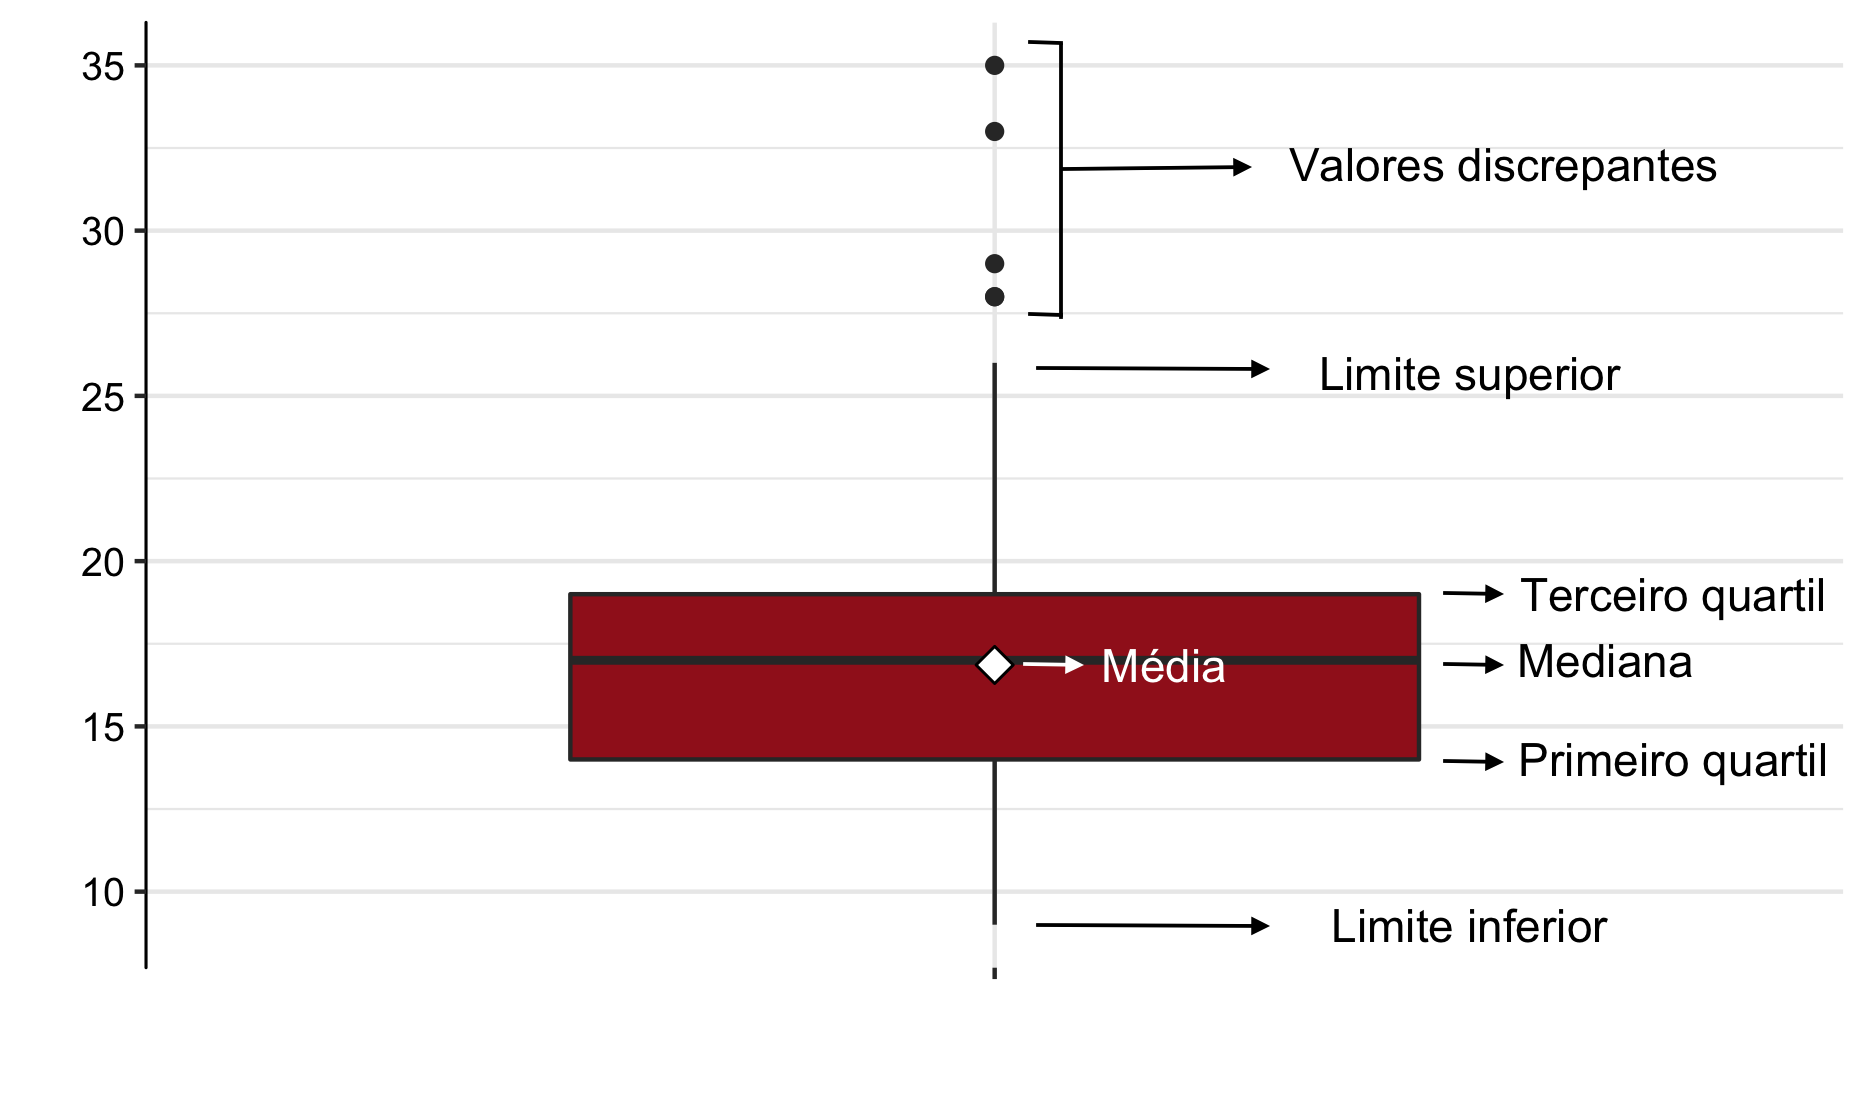
\includegraphics{images/box_uni.png}

}

\end{figure}%

A porção inferior do retângulo diz respeito ao primeiro quartil,
enquanto a superior indica o terceiro quartil. Já o traço no interior do
retângulo representa a mediana do conjunto de dados, ou seja, o valor em
que o conjunto de dados é dividido em dois subconjuntos de mesmo
tamanho. A média é representada pelo losango branco e os pontos são
\emph{outliers}. Os \emph{outliers} são valores discrepantes da série de
dados, ou seja, valores que não demonstram a realidade de um conjunto de
dados.

\subsection{Histograma}\label{histograma}

O histograma é uma representação gráfica utilizada para a visualização
da distribuição dos dados e pode ser construído por valores absolutos,
frequência relativa ou densidade. A figura abaixo ilustra um exemplo de
histograma.

\begin{figure}[H]

\caption{Exemplo de histograma}

{\centering 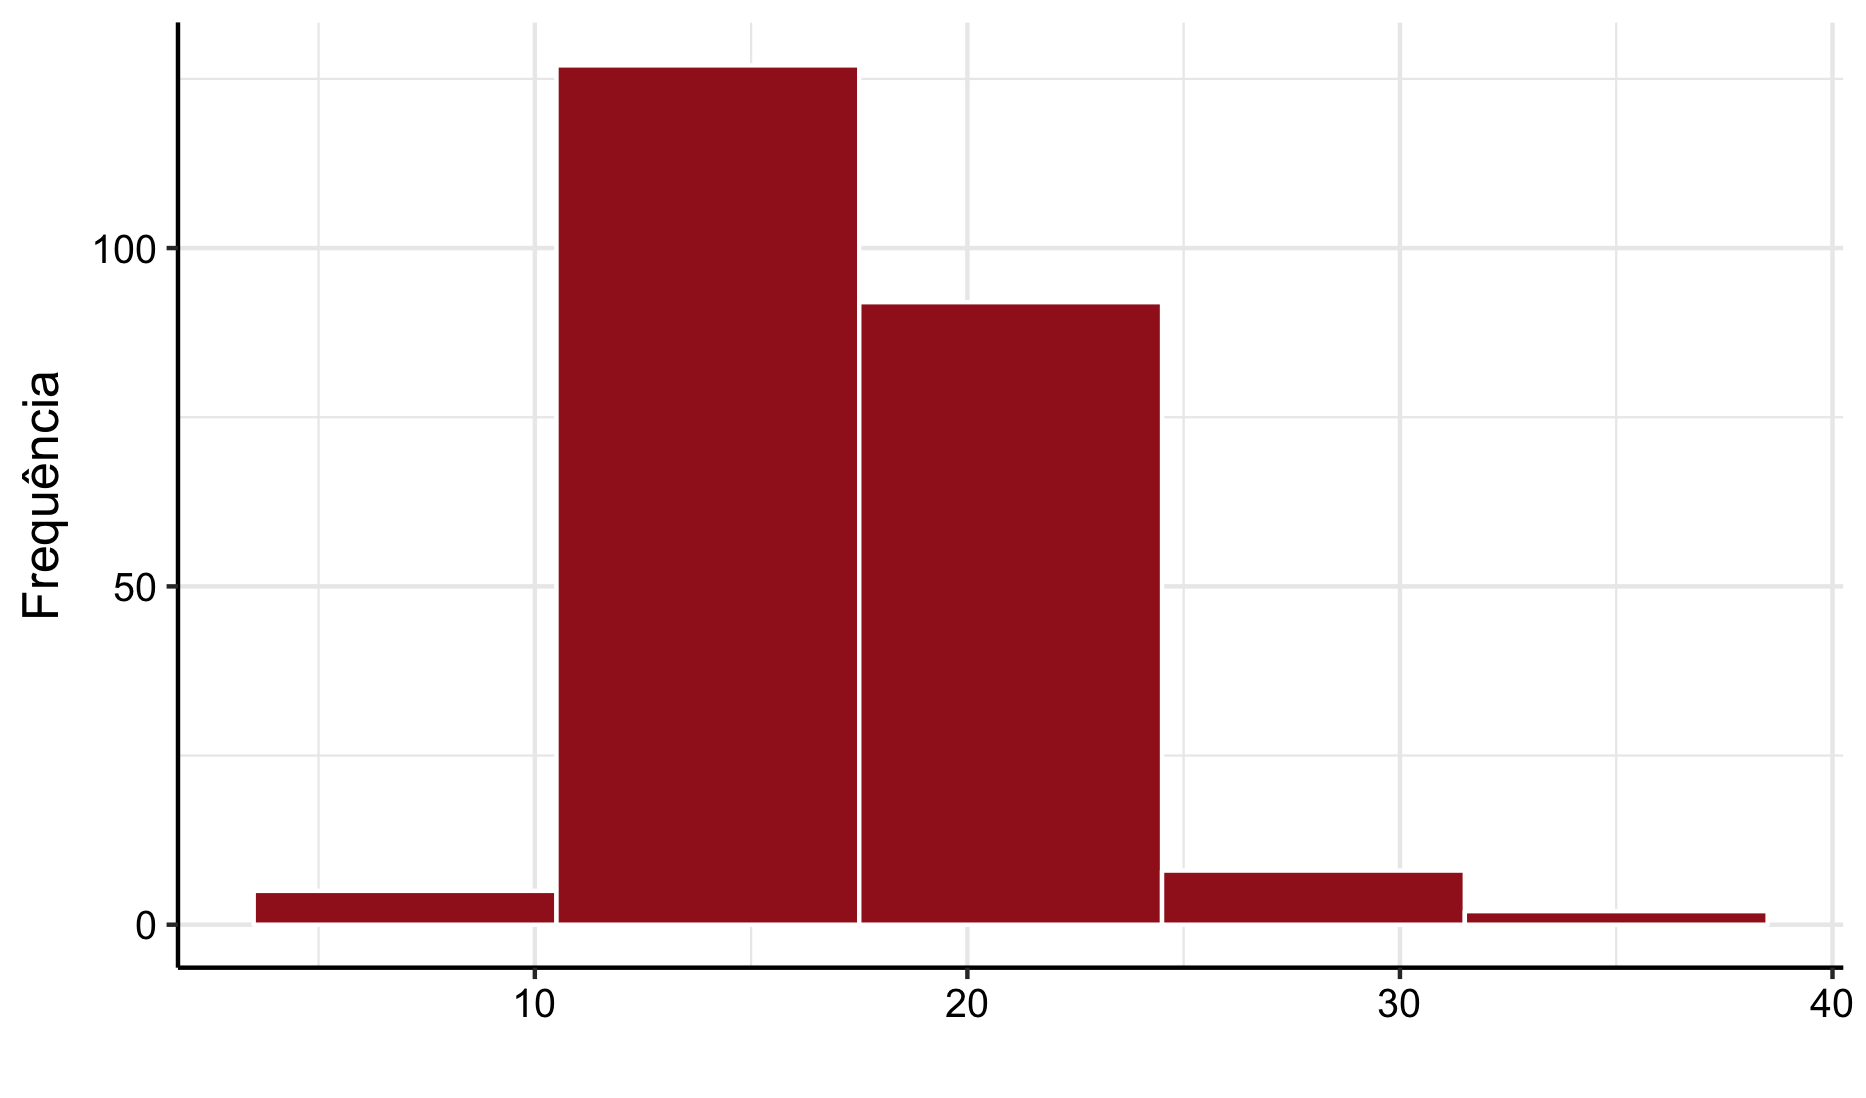
\includegraphics[width=158mm,height=\textheight]{images/hist_uni.png}

}

\end{figure}%

\subsection{Gráfico de Dispersão}\label{gruxe1fico-de-dispersuxe3o}

O gráfico de dispersão é uma representação gráfica utilizada para
ilustrar o comportamento conjunto de duas variáveis quantitativas. A
figura abaixo ilustra um exemplo de gráfico de dispersão, onde cada
ponto representa uma observação do banco de dados.

\begin{figure}[H]

\caption{Exemplo de Gráfico de Dispersão}

{\centering 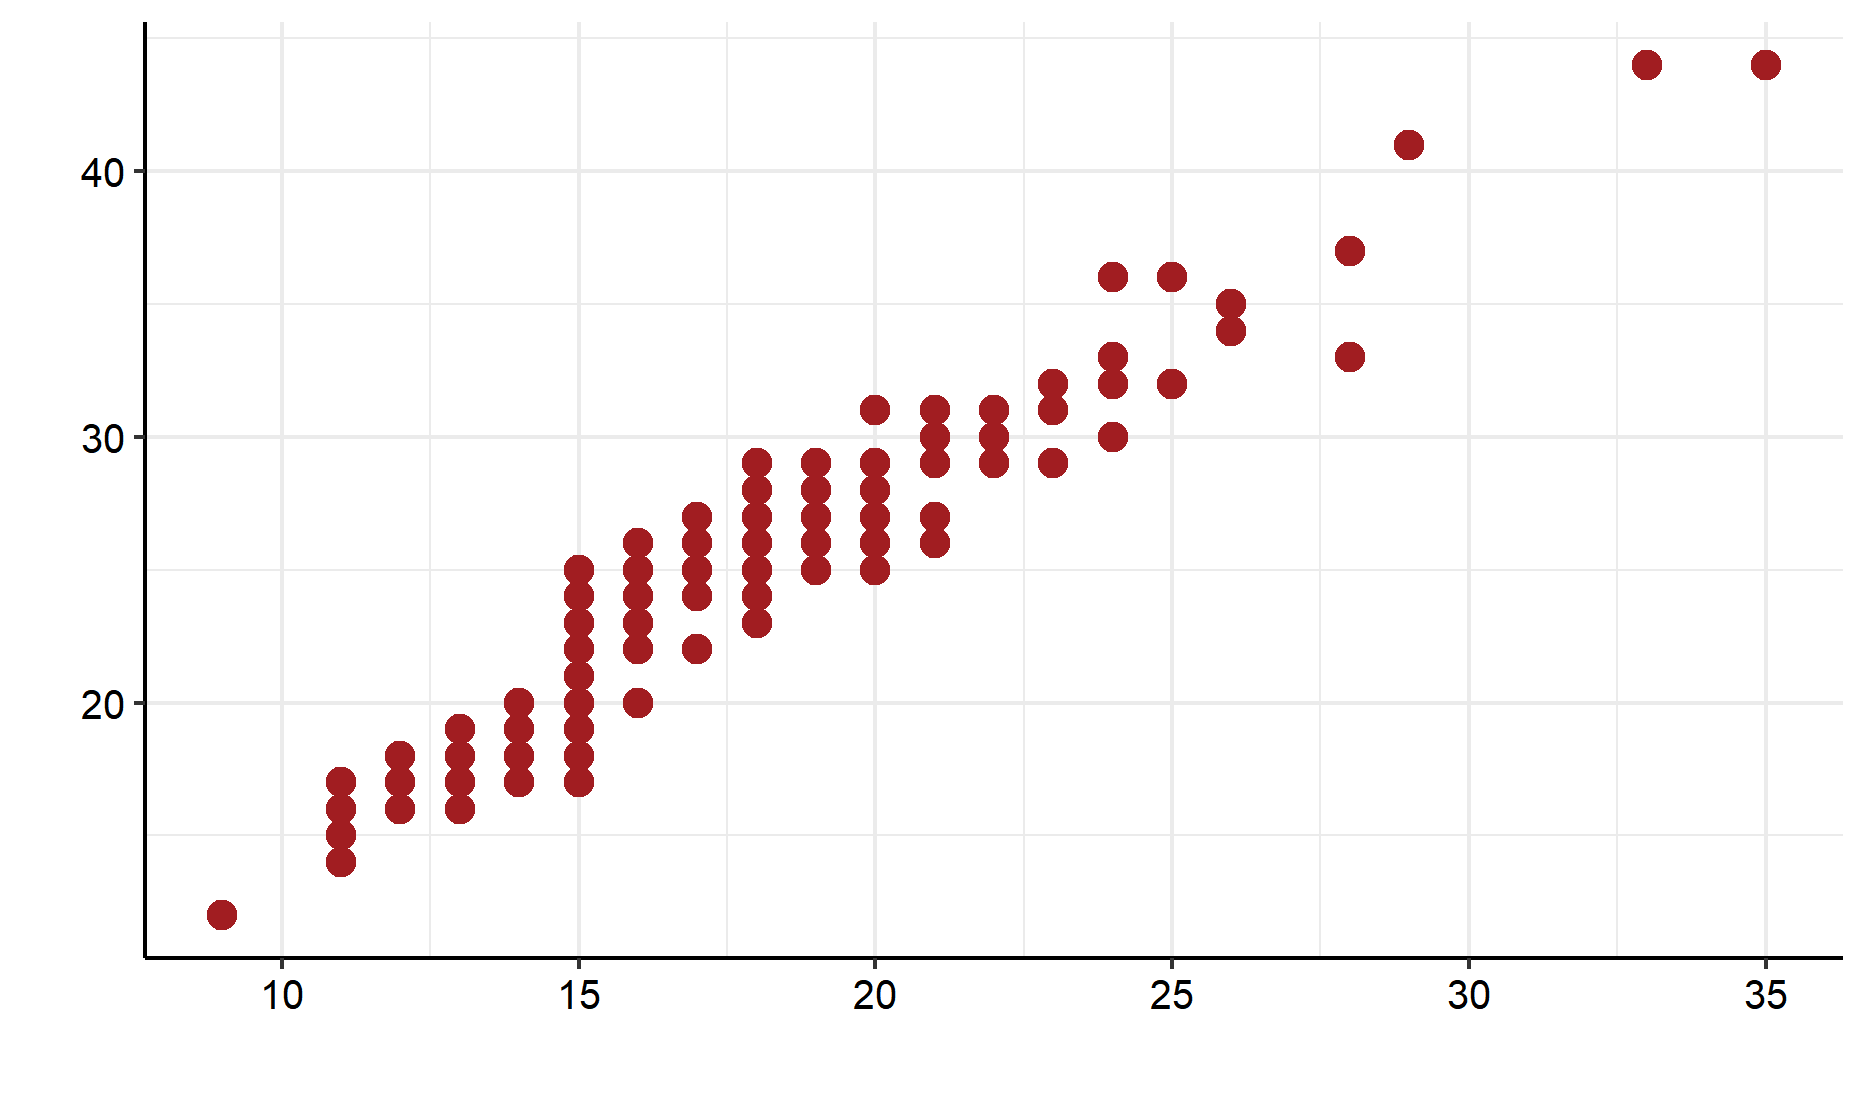
\includegraphics[width=158mm,height=\textheight]{images/disp_uni.png}

}

\end{figure}%

\subsection{Tipos de Variáveis}\label{tipos-de-variuxe1veis}

\subsubsection{Qualitativas}\label{qualitativas}

As variáveis qualitativas são as variáveis não numéricas, que
representam categorias ou características da população. Estas
subdividem-se em:

\begin{itemize}
\tightlist
\item
  \textbf{Nominais}: quando não existe uma ordem entre as categorias da
  variável (exemplos: sexo, cor dos olhos, fumante ou não, etc)
\item
  \textbf{Ordinais}: quando existe uma ordem entre as categorias da
  variável (exemplos: nível de escolaridade, mês, estágio de doença,
  etc)
\end{itemize}

\subsubsection{Quantitativas}\label{quantitativas}

As variáveis quantitativas são as variáveis numéricas, que representam
características numéricas da população, ou seja, quantidades. Estas
subdividem-se em:

\begin{itemize}
\tightlist
\item
  \textbf{Discretas}: quando os possíveis valores são enumeráveis
  (exemplos: número de filhos, número de cigarros fumados, etc)
\item
  \textbf{Contínuas}: quando os possíveis valores são resultado de
  medições (exemplos: massa, altura, tempo, etc)
\end{itemize}

\section{Análises}\label{anuxe1lises}

\subsection{Top 5 países com mais medalhistas
femininas}\label{top-5-pauxedses-com-mais-medalhistas-femininas}

A partir do acesso ao banco de dados disponibilizado pela ``House of
Excellence'', tivemos acesso aos dados de todos os atletas que
participaram das olimpíadas de 2000 até 2016. Nesse cenário, com o
intuito de produzir um ranqueamento das cinco delegações que obtiveram
mais conquistas nesse período nas modalidades femininas, do banco de
dados original, foram utilizadas as variáveis de sexo(``Gender''), a
qual era dividida entre Feminino (``F'') e Masculino (``M''), ainda foi
utilizada a variável que descrevia qual país era a origem do atleta,
sendo a base para agrupar as conquistas, e por último a que evidenciava
qual medalha havia sido conquistada.

\begin{figure}

\caption{\label{fig-prop}Gráfico de colunas do total de conquistas de
cada delegação do Top 5}

\centering{

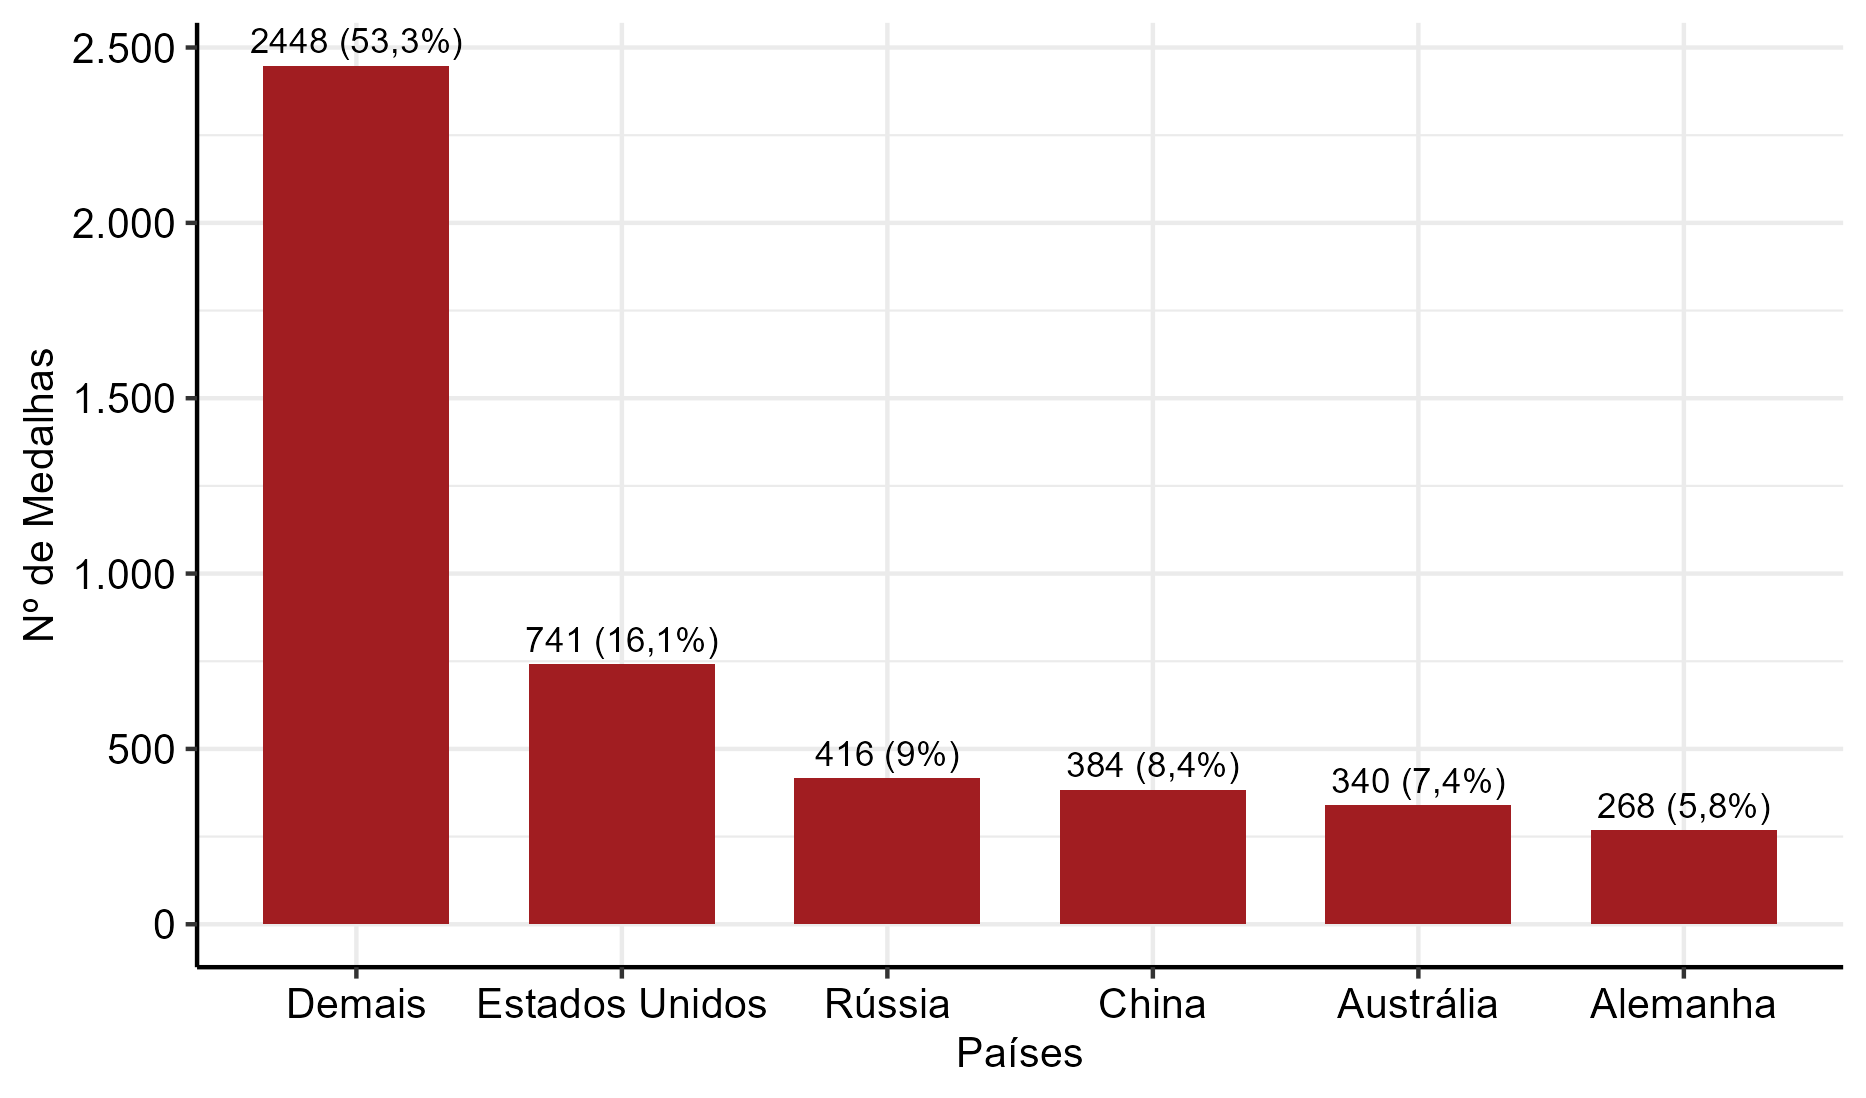
\includegraphics[width=158mm,height=\textheight]{images/colunas-prop-medalha.png}

}

\end{figure}%

Tendo a \ref{fig-prop} como referência podemos analisar que os Estados
Unidos lideram a lista com 741 medalhas, seguidos da delegação russa com
416 - o que representa uma diferença de 325 conquistas entre o primeiro
e o segundo colocado - em terceiro colocado está a China com 384, a
Austrália na quarta posição com 340 e fechando o ranqueamento a Alemanha
com 268, distanciando-se do penúltimo colocado por 72 medalhas e em
relação ao primeiro são 473 - valor maior que as conquistas da Rússia
que ocupa o segundo lugar.

Através da análise dos dados evidencia-se que dentre as modalidades
femininas, durante os anos de 2000 a 2016 considerando todas os pódios
sem distinção entre ouro, prata e bronze, totalizam-se 4597 conquistas.
Dado o interesse da ``House of Excelence'' em entender o cenário das
conquistas olímpicas, foi contruída uma análise da frequência dessas
medalhas em relação ao total de medalhas femininas. Assim por meio da
\ref{fig-prop}, no ``Top 5'' percebe-se que os Estados Unidos detém o
topo do quadro de medalhas com 16,12\%, seguido da Rússia que contém
9,05\% , a China em terceiro com 8,,35\%, a Austrália na quarta posição
com 7,4\% e fechando o ranqueamento a Alemanha com 5,83\%.

\begin{figure}[H]

\caption{\label{fig-setor}Gráfico de setor da frequência de conquistas
entre as delegações dentro e fora do Top 5}

\centering{

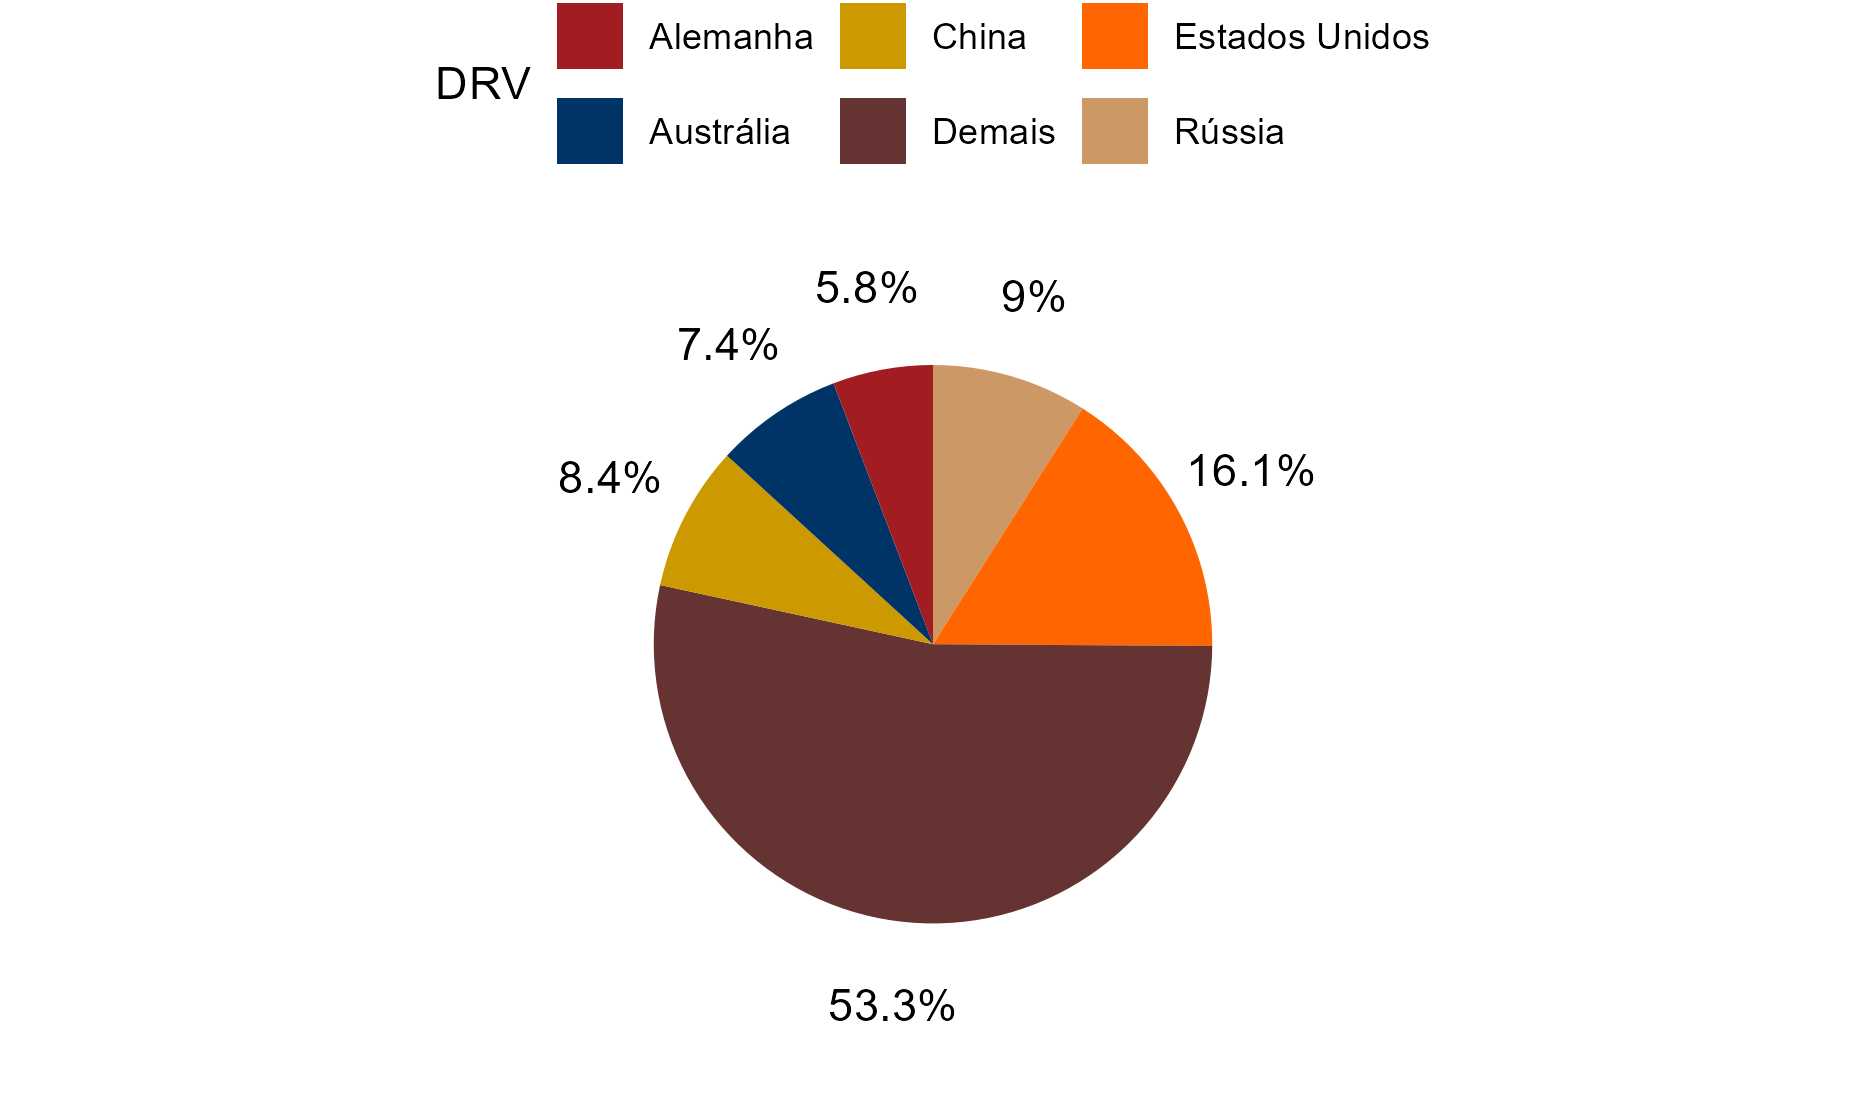
\includegraphics[width=158mm,height=\textheight]{images/setor_paises.png}

}

\end{figure}%

Para mais, a fim de esclarecer como os melhores países se comparam aos
demais, diante da \ref{fig-prop} e da \ref{fig-setor} analisa-se que as
delagações fora do ``Top 5'', totalizam 2448 pódios, o que representa
53,25\% do todo. Nesse cenário, nota-se que os cinco países com melhor
perfomance nos jogos possuem 2149 medalhas, o que condiz a 46,75\% de
todas as conquistas.

\subsection{IMC por Esporte}\label{imc-por-esporte}

Diante do banco de dados, obtivemos acesso às variáveis quantitativas
contínuas que descrevem o peso dos atletas em libras (lbs) e suas
respectivas alturas em metros (m), tendo isso calculamos o Índice de
Massa Corporal (IMC) de cada um dos atletas, atribuindo uma nova
variável ao banco que também é classificada como quantitativa contínua,
para, assim, realizar as análises, além disso, durante os cálculos 22
atletas não tiveram ou suas alturas ou seus pesos computados no banco de
dados e por isso foram retirados da variável que contabiliza todos os
IMC's. Ainda, vale ressaltar que pelo interesse de observar como os
valores de IMC se distribuem, agrupou-se os dados em relação aos
Esportes de interesse, que são identificados como variável qualitativa
nominal, a qual não tem distinção de ordem dentro da categoria, além
disso, tanto homens, quanto mulheres, nesse primeiro momento, foram
agrupados igualmente, conforme suas categorias olímpicas - Atletismo,
Badminton, Futebol, Ginástica, Judô. Posteriormente, terão análises
específicas para o feminino e masculino, mantendo os mesmos esportes de
interesse, ressaltando que o sexo também é uma uma variável qualitativa
nominal.

\begin{figure}

\caption{\label{fig-e-box-expli}Boxplot explicativo sobre seus
elementos}

\centering{

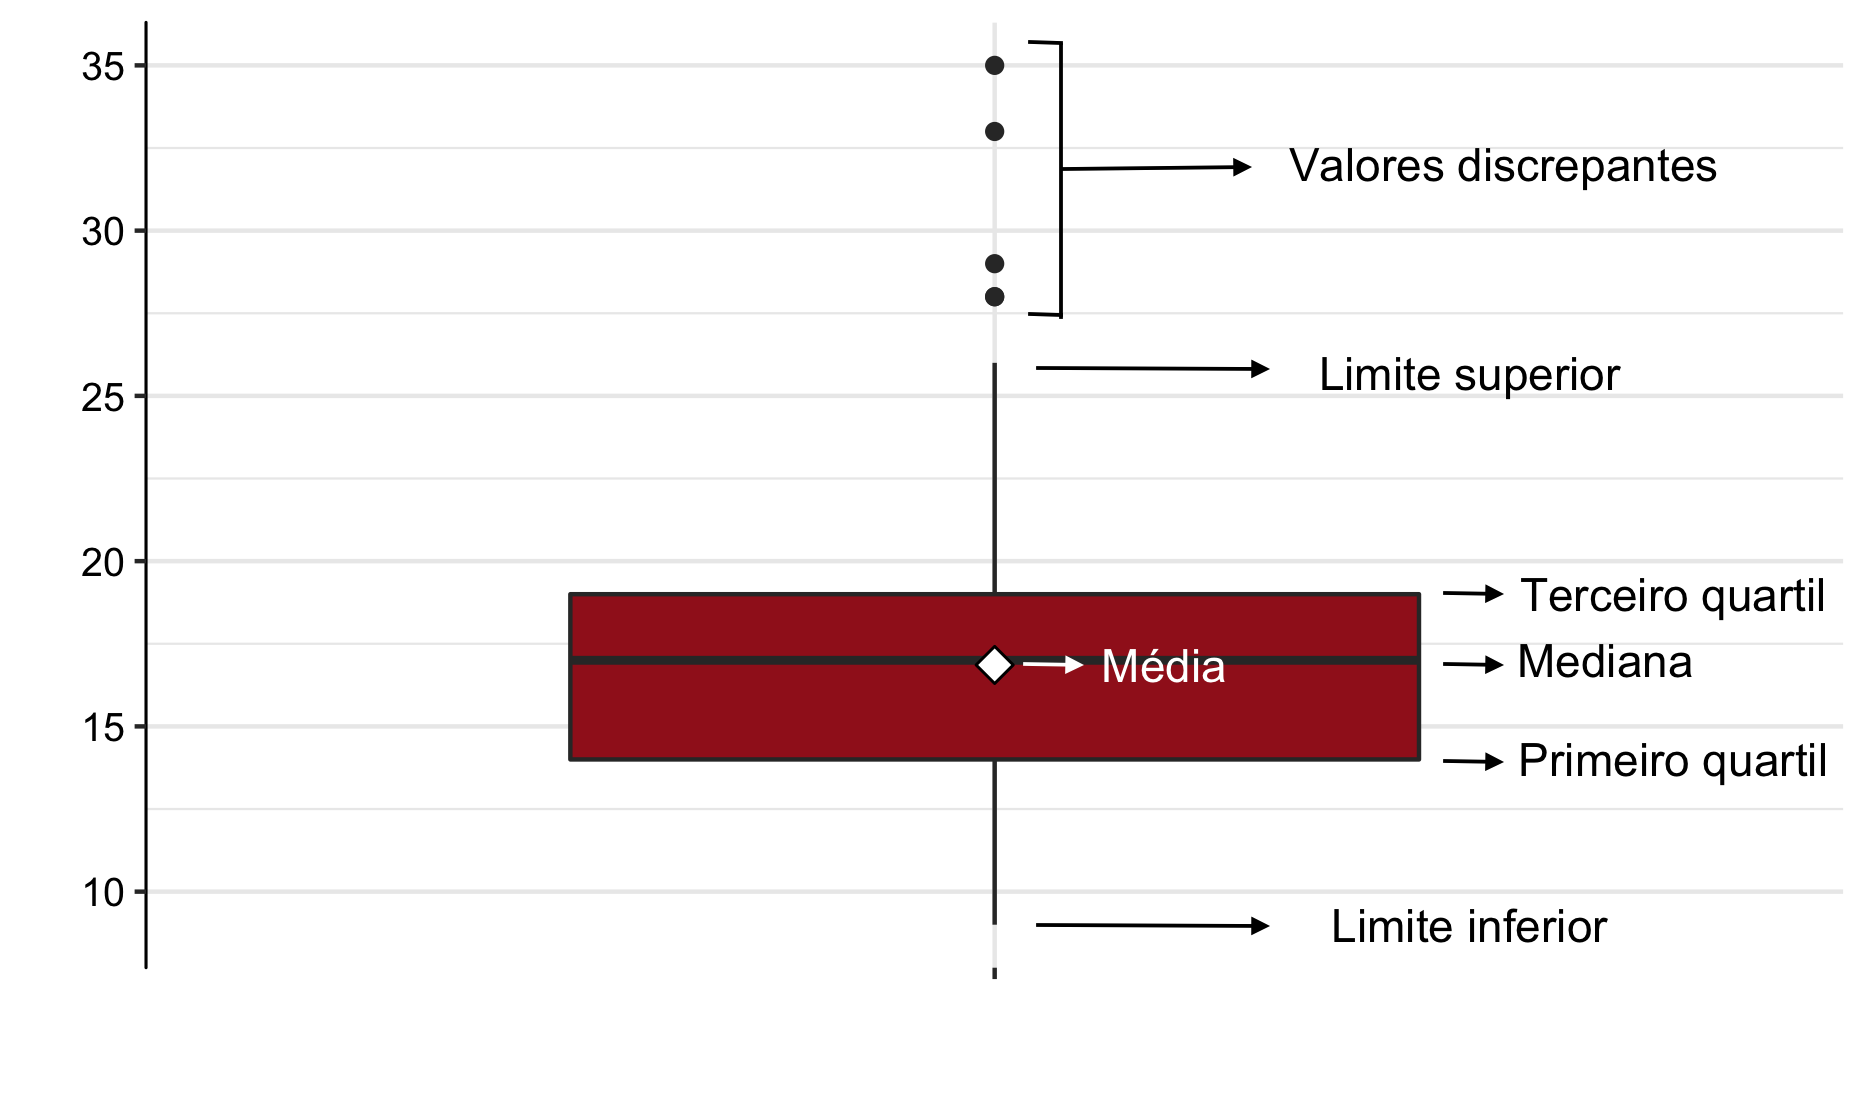
\includegraphics[width=158mm,height=\textheight]{images/box_uni.png}

}

\end{figure}%

Para analisar os dados obtidos utilizaremos \emph{boxplots} como forma
de visualização das informações e por meio da \ref{fig-e-box-expli}
apresenta-se o padrão e estruturação deles.

\begin{figure}[H]

\caption{\label{fig-boxplot}Boxplot dos esportes de interesse pelo IMC}

\centering{

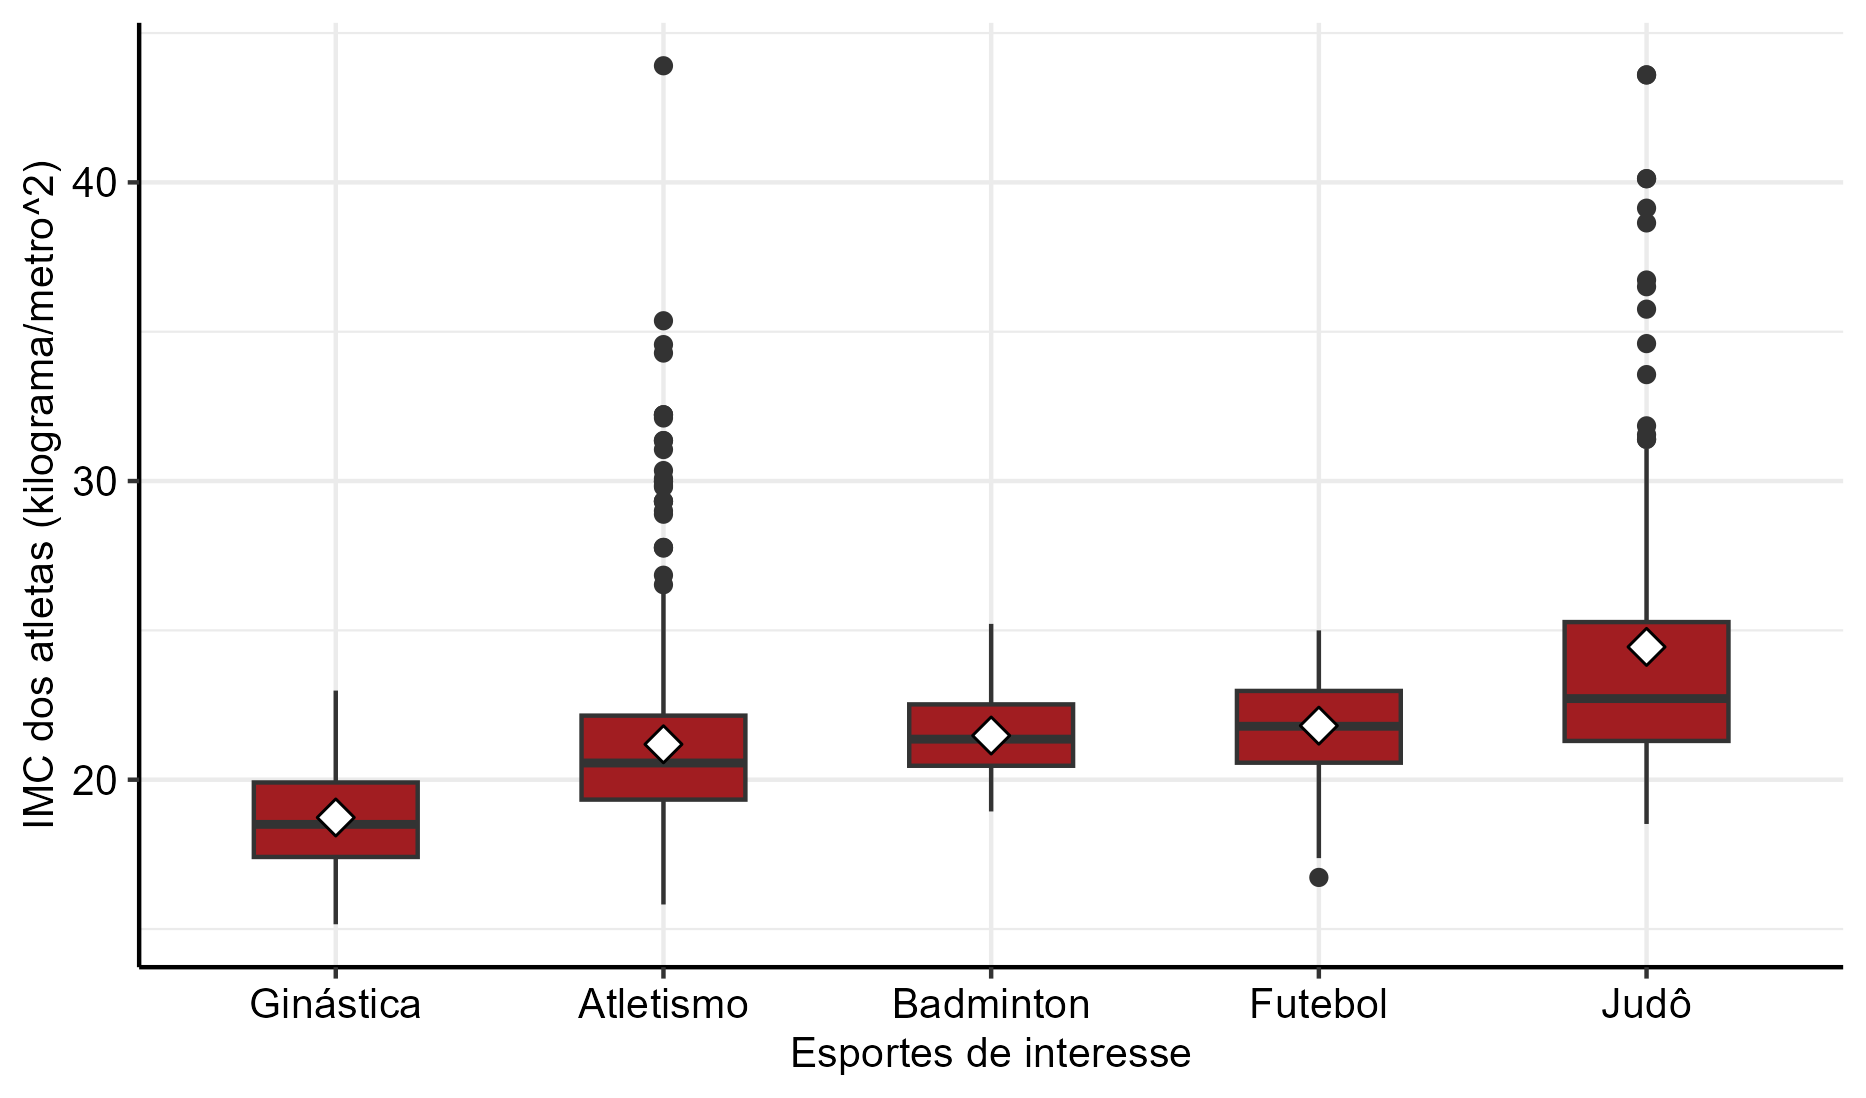
\includegraphics[width=158mm,height=\textheight]{images/box_bi.png}

}

\end{figure}%

\begin{table}[H]

\caption{\label{tbl-medidas}Medidas resumo do IMC por esportes}

\centering{

\begin{tabular}{ | l |
        S[table-format = 2.2]
        S[table-format = 1.2]
        S[table-format = 2.2]
        S[table-format = 2.2]
        S[table-format = 2.2]
        |}
\toprule
    \textbf{Estatística} & \textbf{Atletismo} & \textbf{Badminton} & \textbf{Futebol} & \textbf{Ginástica} & \textbf{Judô} \\
    \midrule
    Média & 22.30 & 22.21 & 22.51 & 20.68 & 25.70 \\
    Desvio Padrão & 3.86 & 1.50 & 1.73 & 2.38 & 5.12 \\
    Variância & 14.92 &  2.26 &  2.99 &  5.67 & 26.23 \\
    Mínimo & 15.82 & 18.94 & 16.73 & 15.16 & 18.52 \\
    1º Quartil & 20.03 & 21.22 & 21.34 & 18.61 & 22.06 \\
    Mediana & 21.45 & 22.28 & 22.49 & 21.09 & 24.68 \\
    3º Quartil & 23.67 & 23.21 & 23.71 & 22.48 & 27.70 \\
    Máximo & 44.38 & 26.73 & 29.07 & 26.45 & 56.50 \\
\bottomrule
\end{tabular}

}

\end{table}%

A partir da \ref{tbl-medidas} e da \ref{fig-boxplot} podemos observar
que o Judô possui maior média de IMC (25,70), isso significa 3,19 a mais
que o segundo colocado - Futebol (22,51) - e maior mediana (24,68) entre
os esportes, esta também é seguida pelo Futebol como segundo maior valor
de mediana entre a população com 22,49, e por outro lado, a Ginástica
tem a menor media (20,68), obtendo um valor mais baixo que quarto menor
IMC médio - Badminton (22,21) - por uma diferença de 1,53, e menor
mediana (21,09) dentre eles, com 0,36 a menos que o Atletismo (21,45).
Além disso, consegue-se perceber que o Badminton possui, dentre os
valores mínimos, o mais alto (18,94), 0,42 a frente do Judô (18,52), e a
Ginástica o mais baixo (15,16), 0,66 a menos que o Atletismo. Já no
quesito de maior valor obtido do índice de massa corporal entre os
atletas está no Judô (56,50), 12,12 a mais que o Atletismo, e a
Ginástica com o menor novamente (26,45), o que representa 0,28 a menos
que Badminton.

Outrossim, observando os valores de 1º Quartil, 3º Quartil, Mediana,
Variância e Desvio Padrão, nota-se que o Badminton e Futebol possuem
valores de IMC mais próximos de primeiro e de terceiro quartil,
evidenciando estarem mais próximos da média, uma vez que a amplitude
interquartílica representa 50\% do total de todas as observações para a
determinada classe. Ainda, percebe-se que para ambos os Esportes suas
medianas, no caso do Badminton (22,28) e do Futebol (22,49) são também
próximos da média, convergindo para o entendimento que há maior
concentração dos valores em torno do valor médio. Sob outra perspectiva,
o Judô é a modalidade que o valores estão mais dispersos na amostra, o
que pode ser percebido pelo maior desvio padrão entre as modalidades
(5,12), assim como a variância (26,23), bem como sua amplitude
interquartil ser a maior entre os demais.

\begin{table}[H]

\caption{\label{tbl-tex}Coeficiente de variação dos esportes de
interesse}

\centering{

\begin{tabular}{l|r}
  \hline
\multicolumn{1}{l|}{\textbf{Esportes}} & \multicolumn{1}{r}{\textbf{Coeficiente de Variação}} \\
  \hline
Atletismo & 17,32\% \\
Badminton & 6,77\% \\
Futebol & 7,68\% \\
Ginástica & 11,51\% \\
Judô & 19,93\% \\
  \hline
\end{tabular}

}

\end{table}%

Antes de analisar a \ref{tbl-tex}, é preciso observar que O coeficiente
de variação auxilia ao fornecer a dispersão dos dados em relação à média
de maneira mais clara, já que seus resultados representam
percentualmente o quanto as classes estão concentradas em torno do valor
médio. De uma maneira mais direta, quanto menor for o seu valor, mais
homogêneos serão os dados, nesse caso homogêneo significa que os valores
não assumem valores dispersos. Portanto, para metrificar o coeficiente
de variação, entende-se como baixo (apontando um conjunto de dados
homogêneo) quando for menor ou igual a 25\%.

Com a \ref{tbl-tex} podemos comprovar o que havia sido analisado
outrora, dentre os demais esportes o que apresenta menor valor para o
Coeficiente de Variação foi o Badminton (6,77\%), ou seja, os atletas
que praticaram essa modalidade durantes as olimpíadas tiveram os valores
de IMC mais homogêneos em relação à média, seguido do Futebol (7,68\%) -
0,91\% de separação entre os dois - com 11,51\% de coeficiente de
variação está a Ginástica que dista 3,83\% do Futebol e possui 5,81\% a
menos de coeficiente que o Atletismo (17,31\%), este se distancia do
Judô (19,93\%) por 2,61\%, evidenciando que o Judô é o que possui os
valores mais dispersos, entretanto ainda se enquadrando como homogêneo.

Dada a consideração de homens e mulheres sem distinção feita
anteriormente, agora abordaremos os resultados para cada gênero
específico, uma vez que, anteriormente, tinhamos um panorama geral, e
neste momento teremos análises mais específicas visando mais eficiência
para os atletas da consultoria esportiva.

\begin{figure}

\caption{\label{fig-box-fem}Boxplot dos esportes de interesse pelo IMC
das atletas femininas}

\centering{

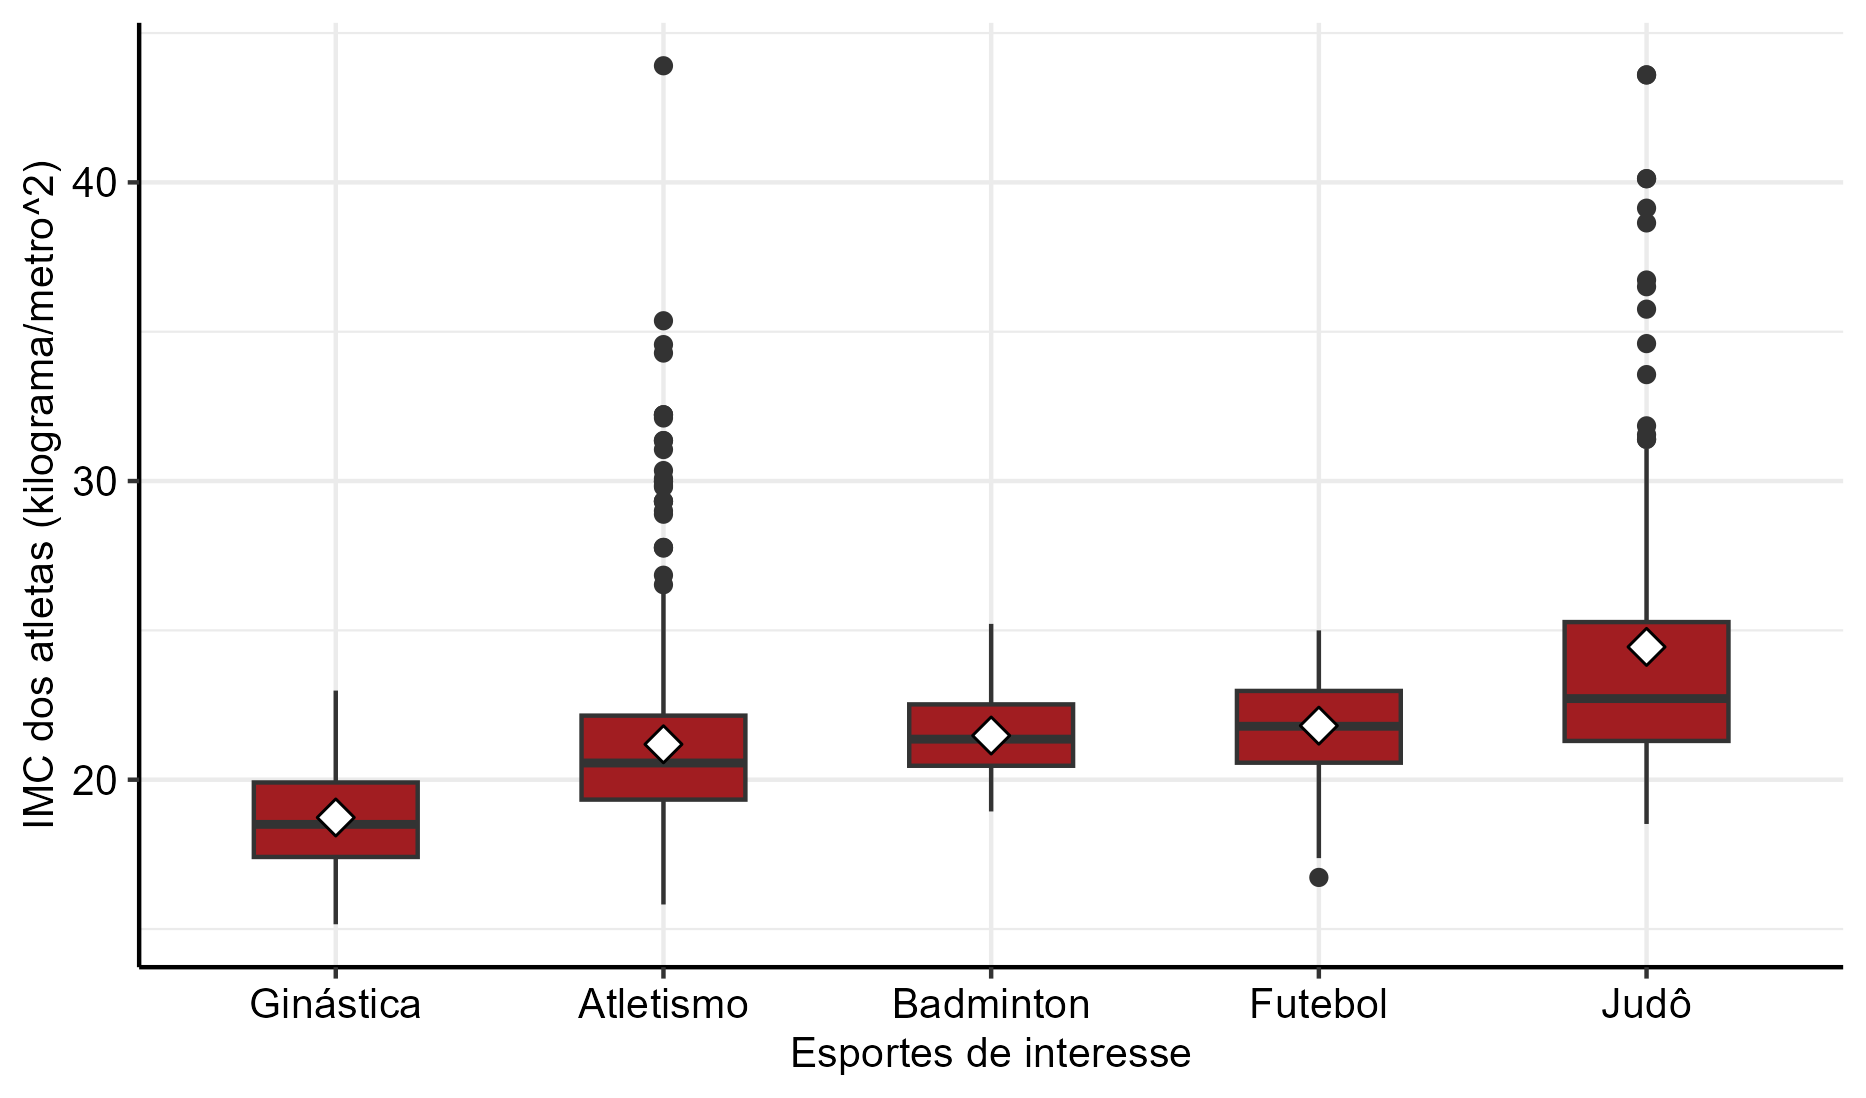
\includegraphics[width=158mm,height=\textheight]{images/box_bi_fem.png}

}

\end{figure}%

\begin{table}[H]

\caption{\label{tbl-medidasfem}Medidas resumo do IMC das atletas
femininas dos esportes de interesse}

\centering{

\begin{tabular}{ | l |
        S[table-format = 2.2]
        S[table-format = 1.2]
        S[table-format = 2.2]
        S[table-format = 2.2]
        S[table-format = 2.2]
        |}
\toprule
    \textbf{Estatística} & \textbf{Atletismo} & \textbf{Badminton} & \textbf{Futebol} & \textbf{Ginástica} & \textbf{Judô} \\
    \midrule
    Média & 21.19 & 21.48 & 21.81 & 18.73 & 24.45 \\
    Desvio Padrão & 3.31 & 1.38 & 1.47 & 1.77 & 5.10 \\
    Variância & 10.98 &  1.91 &  2.16 &  3.12 & 25.98 \\
    Mínimo & 15.82 & 18.94 & 16.73 & 15.16 & 18.52 \\
    1º Quartil & 19.33 & 20.47 & 20.57 & 17.41 & 21.30 \\
    Mediana & 20.56 & 21.36 & 21.79 & 18.50 & 22.72 \\
    3º Quartil & 22.15 & 22.52 & 22.97 & 19.91 & 25.28 \\
    Máximo & 43.90 & 25.22 & 25.00 & 22.98 & 43.60 \\
\bottomrule
\end{tabular}

}

\end{table}%

Antes de analisar os resultados femininos, vale ressaltar que 8 atletas
não haviam os valores necessários no banco de dados para o cálculo do
IMC. Assim, através da \ref{fig-box-fem} e da \ref{tbl-medidasfem},
percebe-se que da mesma forma que a análise generalizada dos gêneros, o
esporte com maior média de IMC foi o Judô (24,45), distanciando 2,64 do
segundo maior que é o Futebol (21,81), assim como o geral, da mesma
forma o Judô também possui a maior mediana com 22,72, 0,93 a mais que
Futebol que ocupa assim como no geral o segundo maior valor de mediana,
porém outrora a ditancia era de 2,19, e a Ginástica possui a menor média
também (18,73), entretanto, nas mulheres, o segundo menor valor de média
é do Atletismo - outrora era do Badminton - com 21,19, uma diferença de
2,46 - distancia maior que no geral, que era de 1,53 entre os dois
menores IMC's médios - já no caso da mediana a Ginástica possui o menor
valor (18,50), 2,06 a menos que o Atletismo (20,56), esses dois esportes
antes estavam distantes por 0,36 e também eram os menores valores de
mediana.

Ademais, observa-se, nos valores mínimos, que as análises femininas são
as mesmas do caso geral, o que nos mostra que os valores de mínimo de
todos os esportes desconsiderando gênero são todos compostos pelos IMC's
de mulheres. Contudo, no panorama dos índices máximos, existem
alterações, analisando o maior valor máximo está o Atletismo (43,90),
seguido do Judô (43,60), diferença de 0,30, diferentememte do caso
geral, o qual era liferado pelo Judô por 12,12 a mais que o Atletismo.
Já nos menores valores de IMC máximo, a Ginástica continua como menor
(22,98), porém agora 2,02 a menos que o quarto menor - Futebol - outra
mudança, posto que antes a distancia era de 0,28 e para o Badminton.

Analisando a distribuição dos dados da população em relação ao valor
médio, nota-se que analisando apenas as mulheres da mesma forma como na
análise geral dos gêneros, o esporte com menor variação dos resultados
de IMC é o badmintos como pode ser percebido pela menor amplitude entre
os quartis (2,05), além de ter os menores valores de desvio padrão
(1,38), além de ter sua mediana (21,36) próxima da média. ALém disso, da
mesma maneira que no caso geral os esportes seguem aquela mesma ordem de
concentração dos valores do índice.

\begin{table}[H]

\caption{\label{tbl-cvfem}Coeficiente de variação de IMC de atletas
femininas dos esportes de interesse}

\centering{

\begin{tabular}{l|r}
  \hline
\multicolumn{1}{l|}{\textbf{Esportes}} & \multicolumn{1}{r}{\textbf{Coeficiente de Variação}} \\
  \hline
Atletismo & 15,64\% \\
Badminton & 6,44\% \\
Futebol & 6,73\% \\
Ginástica & 9,42\% \\
Judô & 20,85\% \\
  \hline
\end{tabular}

}

\end{table}%

Por meio da \ref{tbl-cvfem} conclui-se que o esporte com mais
homogeneidade é de fato o Badminton (6,44\%) - 0,33\% a menos que no
caso geral - e da mesma maneira a segunda modalidade com maior
concentraçâo dos dados em relaçâo à média é o Futebol, entretato agora
com 6,73\%, anteriormente esse valor era de 7,68\% - redução de 0,95\% -
tornando a distância entre Badminton e Futebol de 0,91\% para 0,29\%.
Além disso, na Ginástica a dispersão dos dados mudou, saindo de 11,51\%
e agora atingindo 9,42\%, redução de 2,09\%, diminuição essa, no
coeficiente, que atingiu também o Atletismo antes 17,32\% e no feminino
passou para 15,24\% - 2,08\% de diferença. Contudo, diferentemente dos
demais esportes, o Judô teve acréscimo no valor de coeficiente de
variação, o que indica que os dados passaram a ser mais dispersos, ou
seja mais heterogêneos, para o geral 19,93\% e para as mulheres 20,85\%.

A seguir, encontra-se a análise dos valores de IMC para os homens, no
total forma 14 atletas que não tiveram seus dados computados para o
cálculo do índice da massa corporal.

\begin{figure}[H]

\caption{\label{fig-box-masc}Boxplot dos esportes de interesse pelo IMC
dos atletas masculinos}

\centering{

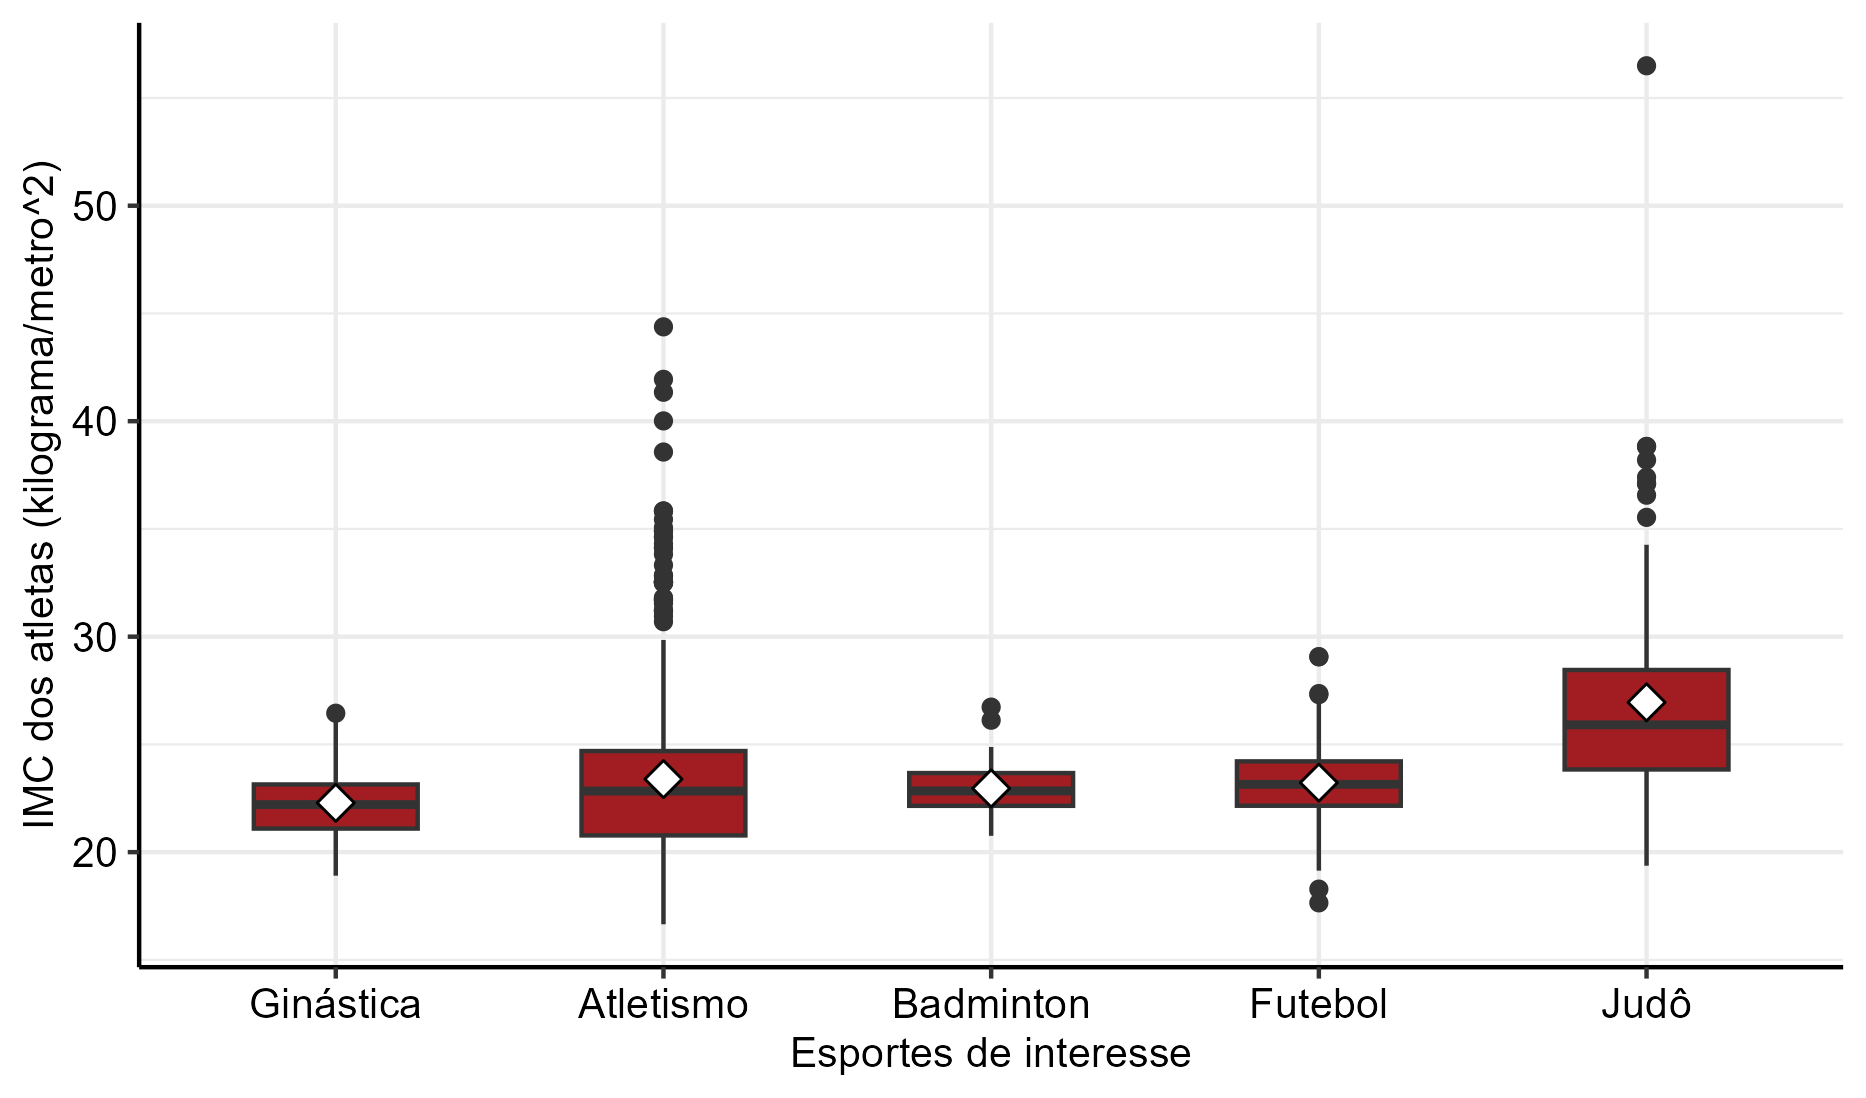
\includegraphics[width=158mm,height=\textheight]{images/box_bi_masc-01.png}

}

\end{figure}%

\begin{table}[H]

\caption{\label{tbl-medidasmasc}Medidas resumo do IMC dos atletas
masculinos dos esportes de interesse}

\centering{

\begin{tabular}{ | l |
            S[table-format = 2.2]
            S[table-format = 1.2]
            S[table-format = 2.2]
            S[table-format = 2.2]
            S[table-format = 2.2]
            |}
    \toprule
        \textbf{Estatística} & \textbf{Atletismo} & \textbf{Badminton} & \textbf{Futebol} & \textbf{Ginástica} & \textbf{Judô} \\
        \midrule
        Média & 23.39 & 22.96 & 23.22 & 22.29 & 26.95 \\
        Desvio Padrão & 4.05 & 1.24 & 1.69 & 1.44 & 4.85 \\
        Variância & 16.39 &  1.53 &  2.84 &  2.06 & 23.51 \\
        Mínimo & 16.65 & 20.76 & 17.65 & 18.91 & 19.37 \\
        1º Quartil & 20.78 & 22.15 & 22.15 & 21.09 & 23.84 \\
        Mediana & 22.84 & 22.84 & 23.15 & 22.21 & 25.91 \\
        3º Quartil & 24.69 & 23.67 & 24.21 & 23.14 & 28.45 \\
        Máximo & 44.38 & 26.73 & 29.07 & 26.45 & 56.50 \\
    \bottomrule
    \end{tabular}

}

\end{table}%

Diante da \ref{fig-box-masc} e da \ref{tbl-medidasmasc}, nota-se que
todas as médias masculinas são maiores que o caso geral, o Judô continua
sendo o maior valor médio (26,95) - o que significa 1,25 a mais - porém
agora não mais seguido pelo Futebol e sim pelo Atletismo (23,39),
distante por 3,56, a diferença entre as duas maiores médias era de 3,19.
No caso do Futebol, agora com 23,22 - 3,62 em relação ao Judô e 0,17 ao
Atletismo, vale ressaltar que essa modalidade tinha média de 22,51
outrora. Por outro lado, nos menores valores médios, a Ginástica
continua como menor (22,29) - 1,61 de acréscimo se comparado com o caso
geral - o que representa uma diferença de 0,67 para o Badminton (22,96),
esse mesmo intervalo era de 1,53.

Para os casos de valor mínimo, também ouve aumento, a categoria que
obteve o mais alto valor mínimo, igualmente ao caso geral está o
Badminton (20,76) - antes de 18,94, acréscimo de 1,82 - seguido do Judô,
da mesma maneira como outrora, com 19,37, 1,39 a menos que o Badminton -
antes era 0,42. Já nos mais baixos valores de mínimo, ocorreram
mudanças, com o Atletismo sendo o menor valor (16,65), antes era a
Ginástica com 15,16, e se distanciando do segundo menor que agora é o
Futebol (17,65) por 1,00, e Ginástica agora com 18,91 - aumento de 3,75.
Para os valores máximos, analogamente, às mulheres que detinham todos os
valores mínimos da análise geral, os homens possuem todos os de máximo.

Ainda, observa-se que o menor desvio padrão continua sendo do Badminton
com 1,24, antes era de 1,50, isso representa alteração de 0,26. No caso
da ginástica que era o terceiro menor, passou a ser o segundo 1,44
diferença de 0,94 ao anterior (2,38) e uma distancia de 0,20 para o
Badminton. Para o Futebol, que era o segundo agora tem desvio padrão de
1,69, mais uma redução em relação ao geral (1,73), mas de 0,04. Para os
mais disperos, aqueles que possuem maior desvio padrão, o Judô continua
como maior valor (4,85) - 0,27 a menos que antes - e 0,80 a mais que o
Atletismo (4,05), essa diferença era de 1,26. Vale ressaltar que maiores
as amplitudes interquartis continuam com o Atletismo (3,91) e Judô
(4,61).

\begin{table}[H]

\caption{\label{tbl-cvmasc}Coeficiente de variação de IMC dos atletas
masculinos dos esportes de interesse}

\centering{

\begin{tabular}{l|r}
  \hline
\multicolumn{1}{l|}{\textbf{Esportes}} & \multicolumn{1}{r}{\textbf{Coeficiente de Variação}} \\
  \hline
Atletismo & 17.31\% \\
Badminton & 5.39\% \\
Futebol & 7.26\% \\
Ginástica & 6.44\% \\
Judô & 17.99\% \\
  \hline
\end{tabular}

}

\end{table}%

A fim de elucidar sobre a homogeneidade dos dados, a \ref{tbl-cvmasc}
mostra que o Badminton (5,39\%), assim como no geral e no feminino, tem
o a menor coeficiente, indicando a maior concentração dos valores em
torno da média, com apenas uma modificação, no masculino a concentração
é a maior entre as demais. Entretanto, diferentemente, do caso geral e
do feminino, o segundo menor valor, no masculno, é da Ginástica
(6,44\%). Outra alteração está no Judô, esse continua sendo o mais
disperso entre as modalidades, o que é percebido pela maior coeficiente,
porém, de todas as análises anteriores, nos homens a categoria obteve a
maior concentração (17,99\%), no caso geral eram 19,93\% e no feminino
20,85\% - o maior valor.

\subsection{3 maiores medalhistas}\label{maiores-medalhistas}

O teste exato de Fisher sugere que os atletas têm uma distribuição
específica de medalhas (ouro, prata, bronze), indicando que alguns
atletas tendem a ganhar mais de um certo tipo de medalha do que outros,
e essa relação não ocorre por acaso.

Essas duas variáveis categóricas formam a tabela de contingência usada
para realizar os testes. No caso do teste exato de Fisher e do teste
qui-quadrado, a ideia é verificar se existe uma associação entre essas
duas variáveis --- ou seja, se o tipo de medalha que um atleta conquista
é independente do atleta, ou se existe uma relação entre o atleta e o
tipo de medalha conquistada. (acho que vou tirar a parte do qui, já que
é impreciso para a baixa frequencia)

\section{Conclusões}\label{conclusuxf5es}




\end{document}
